\documentclass[a4]{article}

\usepackage[left=2cm,right=2cm,top=2cm,bottom=2cm]{geometry} 

\usepackage[utf8]{inputenc}   % otra alternativa para los caracteres acentuados y la "ñ"
\usepackage[           spanish % para poder usar el español
                      ,es-tabla % para los captions de las tablas
                       ]{babel}   
\decimalpoint %para usar el punto decimal en vez de coma para los números con decimales

%\usepackage{beton}
%\usepackage[T1]{fontenc}

\usepackage{parskip}
\usepackage{xcolor}

\usepackage{caption}

\usepackage{enumerate} % paquete para poder personalizar fácilmente la apariencia de las listas enumerativas

\usepackage{graphicx} % figuras
\usepackage{subfigure} % subfiguras

\usepackage{amsfonts}
\usepackage{amsmath}

\definecolor{gris}{RGB}{220,220,220}
	
\usepackage{float} % para controlar la situación de los entornos flotantes

\restylefloat{figure}
\restylefloat{table} 
\setlength{\parindent}{0mm}


\usepackage[bookmarks=true,
            bookmarksnumbered=false, % true means bookmarks in 
                                     % left window are numbered
            bookmarksopen=false,     % true means only level 1
                                     % are displayed.
            colorlinks=true,
            allcolors=blue,
            urlcolor=cyan]{hyperref}
\definecolor{webblue}{rgb}{0, 0, 0.5}  % less intense blue


\title{Aprendizaje Automático: Proyecto Final \\ Devanagari Handwritten Characters}

\author{David Cabezas Berrido y Patricia Córdoba Hidalgo}

\date{}

\begin{document}

\maketitle
\tableofcontents

\newpage

\section{Problema}

El problema a resolver consiste en clasificar caracteres de la
escritura Devanagari. Nuestros datos son imágenes de estos símbolos
escritos a mano, cada uno de ellos con una etiqueta especificando el
símbolo que representa la imagen.

Inicialemente, nuestro espacio de características $\mathcal{X}$ está
formado por imágenes de $32 \times 32$ píxeles cada una, con un marco
de $2$ píxeles por cada uno de los $4$ lados. El conjunto de
etiquetas, $Y$ son los $46$ caracteres que consideramos, $36$ letras y
$10$ dígitos (del $0$ a $9$). La función objetivo $f$ que buscamos
aproximar es aquella que a una cuadrícula de píxeles representando un
símbolo Devanagari manuscrito le haga corresponder la clase del
símbolo correspondiente.

\section{Dataset. Conjuntos de train y test}

El conjunto de datos de los que disponemos \\
\href{https://archive.ics.uci.edu/ml/datasets/Devanagari+Handwritten+Character+Dataset}{https://archive.ics.uci.edu/ml/datasets/Devanagari+Handwritten+Character+Dataset}
consta de 92000 instancias (imágenes etiquetadas), 2000 de cada una de
las 46 clases. Los datos vienen divididos en train: 78200 instancias
(85\%), 1700 por clase; y test: 13800 instancias (15\%), 300 por
clase. No existen datos perdidos y las clases están perfectamente
balanceadas.

Existen algunos artículos y proyectos relativos a este dataset, por lo
que mantener esta división entre train y test nos permitirá
comparar los resultados que logren nuestros modelos y procesamiento
con los resultados de otros diseñados por terceros. 

En la descripción del dataset se informa de que estos datos proceden
de documentos escritos, pero desconocemos su procedencia y sus
autores. En problemas de reconocimiento de símbolos manuscritos existe
la dificultad de que un modelo aprenda a reconocer símbolos de un
único autor o un conjunto de autores, lo que conlleva sobreajuste y a
estimaciones por validación poco fiables, ya que la muestra de
entrenamiento no termina de ser representativa y el modelo se adapta a
ese sesgo. En nuestro caso, desconocemos si los datos de train y test
corresponden a símbolos trazados por distintas personas o no, con lo
que tenemos otra razón más para respetar la partición de conjuntos de
train y test existente.

Extraemos un conjunto de validación del 20\% de los datos de
entrenamiento para consultar la eficacia práctica de ciertas
decisiones que tomamos durante el preprocesamiento. Esto nos deja con
62560 (80\%) datos para entrenar cada alternativa y 15640 datos para
validar. Debido a la abundancia de datos, podemos esperar que los
scores obtenidos al validar sean representativos de la bondad real de
un modelo o procesamiento, así que decidimos no usar validación
cruzada, ya que es computacionalmente muy costosa y el ajuste de los
modelos es lento debido a la cantidad de datos.

Para ello usamos la función \texttt{train\_test\_split} de
\textit{sklearn} e indicamos mediante la opción \texttt{stratify} que
queremos preservar la proporción de elementos de cada clase en cada
uno de los conjuntos, de forma que sigan perfectamente balanceadas.

\subsection{Formato de los datos}

En el fichero \texttt{png\_to\_np.py}, guardamos las imágenes,
originalmente en formato \texttt{png}, como array. Para ello leemos
cada imagen como array de escala de grises usando la función
\texttt{imread} de \textit{matplotlib} y eliminamos los dos píxeles de
marco por cada lado, quedándonos con matrices de $28 \times 28$ de
valores flotantes entre $0$ y $1$ representando la intensidad de gris
en cada pixel. El resultado es guardado en disco, lo hacemos con la
función \texttt{saveGrey}, que usa la función
\texttt{savez\_compressed} de \textit{numpy} para almacenarlo en
formato \texttt{npz}.

Este fichero solo se ejecuta una vez para cambiar el formato de los
datos. Tras esto, podemos usar los datos guardados en disco para las
sucesivas ejecuciones del código. Proporcionamos los datos ya
transformados, aunque en el fichero \texttt{main.py} se puede alterar
la variable \texttt{PNG\_TO\_NP} para ejecutar el script que carga las
imágenes y almacena estos datos en disco.

\section{Preprocesamiento}

% Comentar justificaciones: 3 modelos ajustados con parámetros por defecto. WIDTH y BLOCK_REDUCE

El preprocesamiento se realiza
imagen a imagen, siendo el resultado sólo dependiente de la propia
imagen y por tanto paralelizable. Para cada imagen realizamos dos operaciones: centrado y reescalado, y downsampling. Tras este proceso, nos quedan $196$ características ($14 \times 14$) y comprobamos con la función \texttt{VarianceThreshold} de \textit{sklearn} que no hay características con varianza $0$ en el conjunto de train (todas aportan algo de información). Consideramos que no es necesario normalizar las variables, ya que todas tienen la misma naturaleza (intensidad de gris en un píxel) y la misma escala (entre $0$ y $1$).

\subsection{Centrado y reescalado}

Esta operación la realiza la función \texttt{centerAndResize}. Ante
una imagen, calculamos un umbral con la ayuda del \href{https://en.wikipedia.org/wiki/Otsu%27s_method}{método de Otsu}
  para
\href{https://en.wikipedia.org/wiki/Thresholding_(image_processing)}{thresholding} (usando la función \texttt{threshold\_otsu} de la librería \textit{skimage}). 

Para calcular la caja englobante del carácter, usamos el
\href{https://en.wikipedia.org/wiki/Closing_%28morphology%29}{closing}
  (función \texttt{closing} de \textit{skimage}) de la imagen
  resultante de considerar los píxeles con intensidad superior a este
  umbral. Recortamos el exterior de la caja y reescalamos la imagen a
  \texttt{WIDTH $\times$ WIDTH} para trabajar con un tamaño de imagen
  unificado (función \texttt{resize} de \textit{skimage}).


\begin{figure}[H]
  \centering
  \subfigure[Muestra antes del preprocesado]{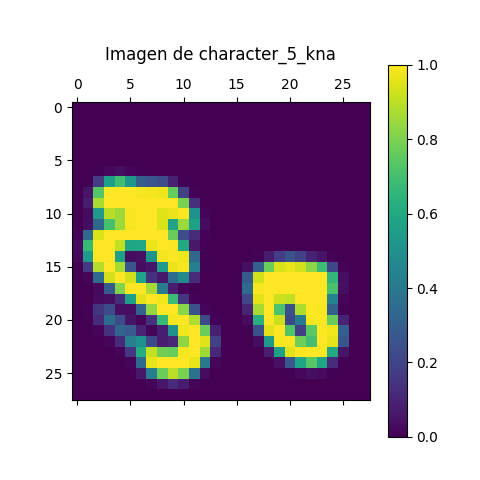
\includegraphics[width=87mm]{imgs/sample-kna.png}}
  \subfigure[Thresholding y closing]{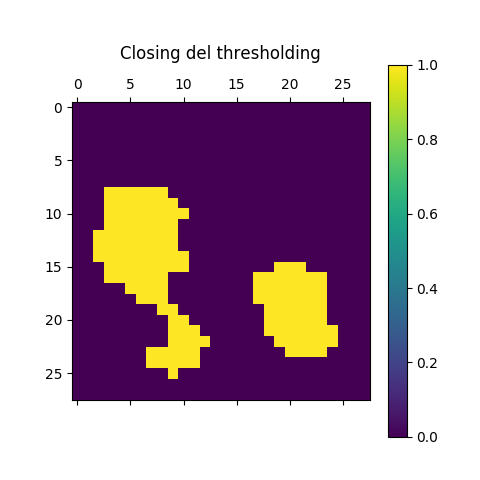
\includegraphics[width=87mm]{imgs/closing-thresholding.png}}
  \subfigure[Recortado de la caja englobante]{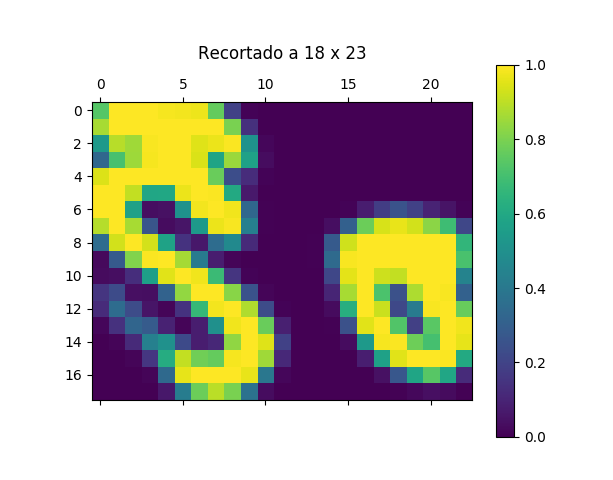
\includegraphics[width=87mm]{imgs/crop.png}}
  \subfigure[Reescalado]{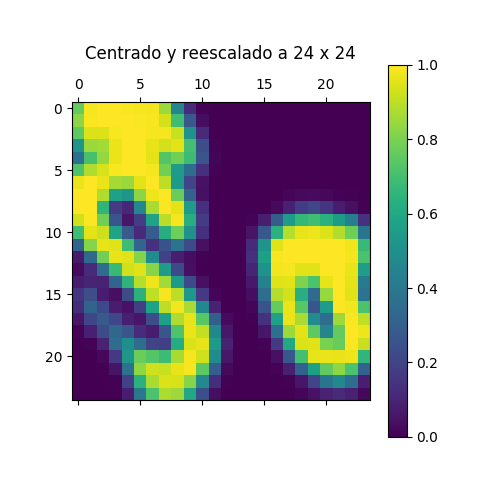
\includegraphics[width=87mm]{imgs/resize.png}}
  \caption{Proceso de centrado y reescalado sobre una instancia correspondiente al carácter kna\\ (usando \texttt{WIDTH} = 24)}
  \label{fig:centerAndResize}
\end{figure}

\subsection{Downsampling}

Para reducir la dimensionalidad, realizamos un downsampling o
reducción por bloques de la imagen, agrupando cada bloque de 4
píxeles en uno usando la media de sus valores. Esta reducción se lleva
a cabo con la función \texttt{block\_reduce} de \textit{skimage}.

\begin{figure}[H]
  \centering
  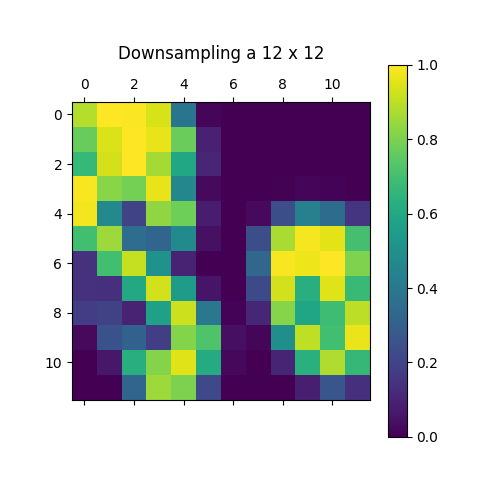
\includegraphics[width=87mm]{imgs/downsampling.png}
  \caption{Resultado del preprocesamiento (tras combinar centrado y reescalado con downsampling usando\\ \texttt{WIDTH} = 24)}
  \label{fig:downsampling}
\end{figure}

\subsection{Utilidad del preprocesamiento}

Queremos comprobar que el preprocesamiento que hemos realizado
realmente ayudará al posterior entrenamiento de los modelos y mejorará
los resultados. Usando los 3 modelos escogidos para el ajuste con sus
respectivos hiperparámetros previamente seleccionados (hablaremos de
esto más detenidamente en secciones posteriores) veremos la accuracy
obtenida sobre nuestro subconjunto de validación en cada una de las
siguientes comparaciones.

Durante el preprocesamiento, hemos tomado dos decisiones que podrían
afectar al desempeño posterior de los modelos. Esas dos decisiones
son: el valor de la variable \texttt{WIDTH} y usar o no
\texttt{block\_reduce} para reducir la dimensionalidad.

Para el valor de la variable \texttt{WIDTH} hemos consderado $28$, ya
que muchos caracteres ocupan toda la imagen y no se llegan a recortar,
y $24$, para intentar encontrar un tamaño intermedio entre las que se
recortan y las que no.

La decisión de reducir dimensionalidad con \texttt{block\_reduce} es
arriesgada porque se produce una pérdida de información de los
datos. Tenemos que contrastar si esa pérdida de información es
significativa atendiedo a las ventajas que supone hacerla: simplifica
el problema (menor dimensionalidad) y reduce los tiempos de ejecución.

Los resultados obtenidos son (con \texttt{block\_reduce}=True):

\begin{center}
\begin{tabular}{|c|c|c|}
\hline
\multicolumn{1}{|c|}{Modelos}& \textbf{\texttt{WIDTH} = 28} &
\textbf{\texttt{WIDTH} = 24}  \\ \hline
  Random Forest         & 0.9195652173913044 & 0.9117647058823529 \\
  Multilayer Perceptron & 0.8879156010230179 & 0.885230179028133 \\
  Regresión Logística   & 0.7273657289002557 & 0.7289002557544757 \\
  Media (no lineales) & 0.903740409 & 0.898497442 \\
  Media & 0.844948849 & 0.841965047 \\ \hline
\end{tabular}
\end{center}

Los resultados obtenidos son (con \texttt{block\_reduce}=False):

\begin{center}
\begin{tabular}{|c|c|c|}
\hline
\multicolumn{1}{|c|}{Modelos}& \textbf{\texttt{WIDTH} = 28} &
\textbf{\texttt{WIDTH} = 24}  \\ \hline
  Random Forest         & 0.9115728900255754 & 0.9159846547314578 \\
  Multilayer Perceptron & 0.8574168797953964 & 0.8688618925831202 \\
  Regresión Logística   & Error de memoria   & Error de memoria \\
  Media (no lineales) & 0.884494885 & 0.892423274 \\ \hline
\end{tabular}
\end{center}

A la vista de los resultados obtenidos, hemos decidido que merece la
pena usar \texttt{block\_reduce}. El valor de \texttt{WIDTH} que
elegimos es $28$. Esta configuración presenta la mayor media y el
mayor máximo de las accuracy en las validaciones de los modelos.

Los resultados tras el preprocesamiento comparándolos con los datos en crudo son:
\begin{center}
\begin{tabular}{|c|c|c|}
  \hline
  \multicolumn{1}{|c|}{Modelos}& \textbf{Antes del preprocesamiento} &
                                                                       \textbf{Después del preprocesamiento}  \\ \hline
  Random Forest         & 0.9070971867007672 & 0.9195652173913044 \\
  Multilayer Perceptron & 0.8464194373401535 & 0.882161125319693 \\
  Regresión Logística   & Error de memoria   & 0.7273657289002557 \\ \hline
\end{tabular}
\end{center}

Podemos observar que con el preprocesamiento hemos conseguido reducir
notablemente la dimensionalidad del problema: pasando de
$28\times 28=784$ variables a $14\times 14=196$. Además, mejoramos en
cierta medida la precisión de los modelos.

\section{Visualización de los datos mediante proyección 2D}

Podemos proyectar los datos en dos dimensiones para intuir de un
simple vistazo hasta que punto la información de la que disponemos nos
permitirá discernir unas clases de otras, y así conocer (entre otras
cosas) si se ha perdido información durante el
preprocesamiento. Existen algoritmos para esto: PCA (Principal
Component Analysis), que proyecta las dos direcciones que más nos
ayuden a discernir los datos. También TSNE (T-distributd Stochastic
Neighbor Embedding), un algoritmo iterativo (lo lanzamos con la salida
de PCA como proyección inicial) que proyecta los datos en dos
dimensiones de forma que para cada dato sus vecinos más cercanos
queden proyectados cerca.

El gran número de datos hace que estas representaciones tarden mucho
tiempo en generarse y estén muy cargadas, por lo que sólo
representamos el 40\% de los datos (elegidos aleatoriamente). Para
ellod usamos la función \texttt{train\_test\_split} de
\textit{sklearn} e indicamos mediante la opción \texttt{stratify} que
queremos preservar la proporción de elementos de cada clase en cada
uno de los conjuntos, de forma que sigan perfectamente
balanceadas. Debido a la abundancia de datos, este 40\% es
suficientemente representativo de la distribución de los datos.

Además, debido al elevado número de clases, no podemos representar
cada un con un color diferente de forma que sean fácilmente
distinguibles, por eso las representamos separadas en 3 gráficas
diferentes: caracteres del 1 al 18, caracteres del 19 al 36 y dígitos
(del 0 al 9). Nos interesa ver si las instancias de la misma clase
están cerca entre sí, no la localización en el espacio. Por tanto
omitimos la leyenda (que además sería extremadamente larga y taparía
el gráfico).

Generamos estas representaciones antes y después del preprocesado,
para advertir si la reducción de dimensionalidad conlleva una pérdida
considerable de información.

\begin{figure}[H]
  \centering
  \subfigure[PCA. Con preprocesamiento]{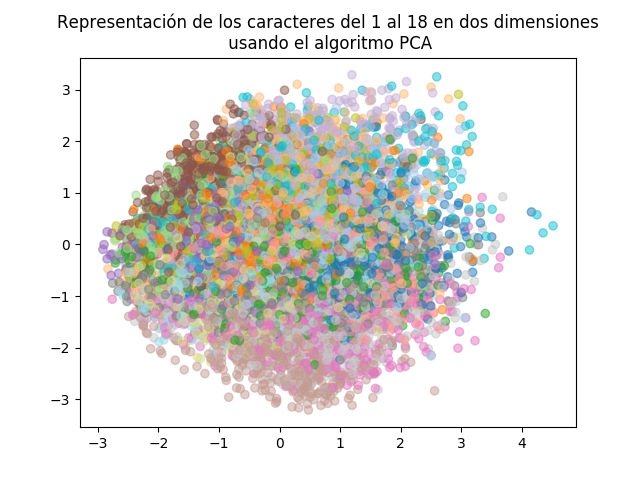
\includegraphics[width=60mm]{imgs/pca1}}
  \subfigure[PCA. Sin preprocesamiento]{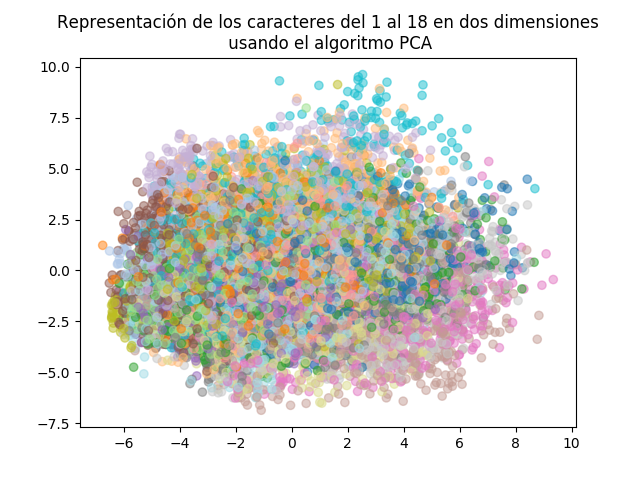
\includegraphics[width=60mm]{imgs/pca-nopre1}}
  \subfigure[TSNE. Con preprocesamiento]{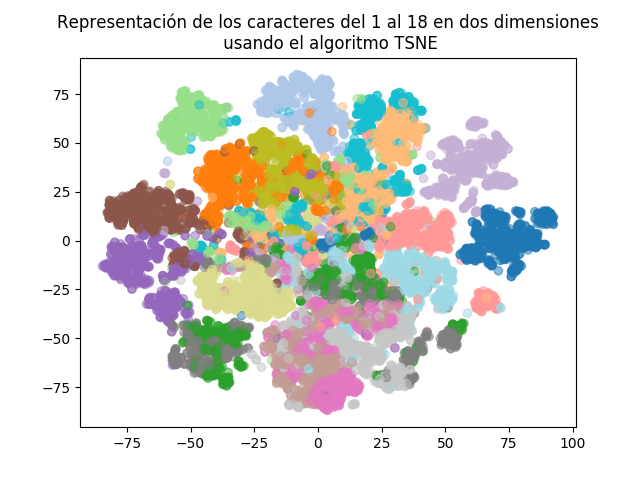
\includegraphics[width=60mm]{imgs/tsne1}}
  \subfigure[TSNE. Sin preprocesamiento]{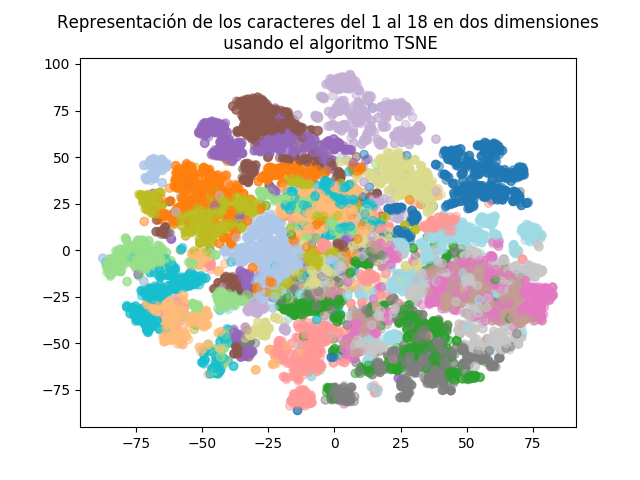
\includegraphics[width=60mm]{imgs/tsne-nopre1}}
  \caption{Proyecciones en 2D de las clases correspondientes a los caracteres del 1 al 18}
  \label{fig:char1-18}
\end{figure}

\begin{figure}[H]
  \centering
  \subfigure[PCA. Con preprocesamiento]{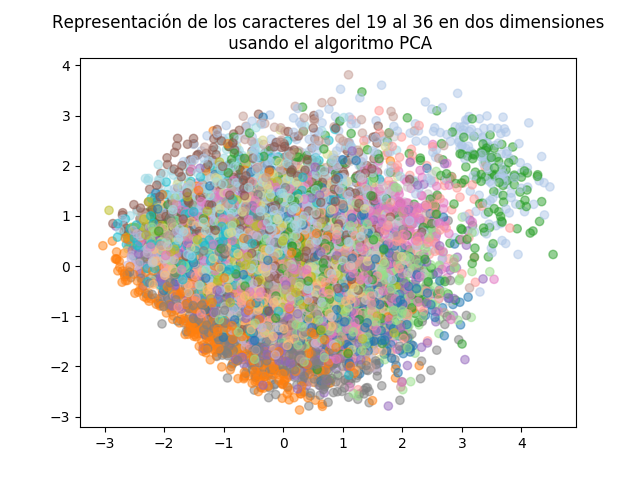
\includegraphics[width=60mm]{imgs/pca2}}
  \subfigure[PCA. Sin preprocesamiento]{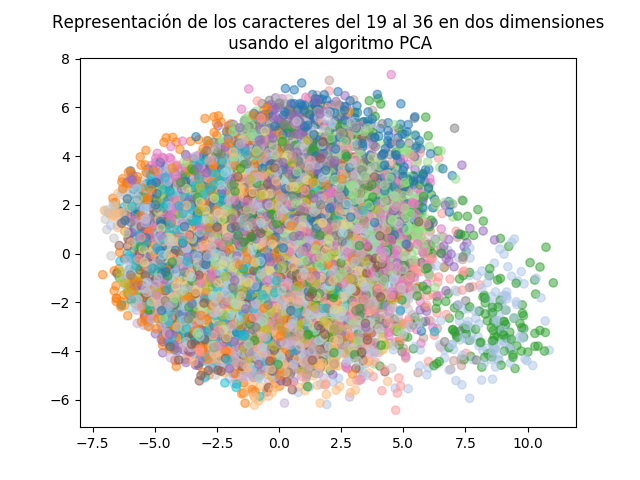
\includegraphics[width=60mm]{imgs/pca-nopre2}}
  \subfigure[TSNE. Con preprocesamiento]{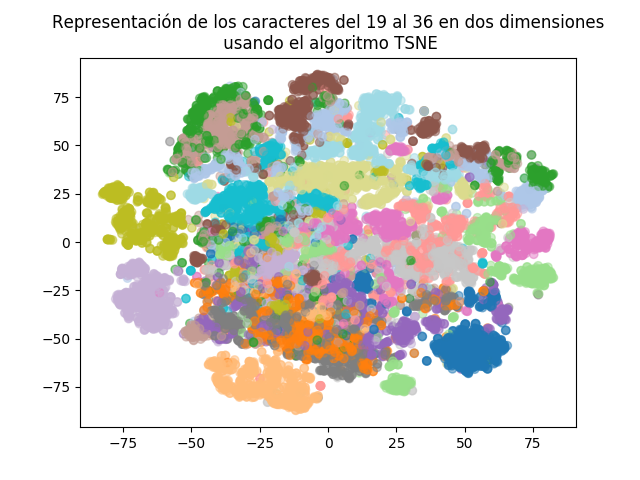
\includegraphics[width=60mm]{imgs/tsne2}}
  \subfigure[TSNE. Sin preprocesamiento]{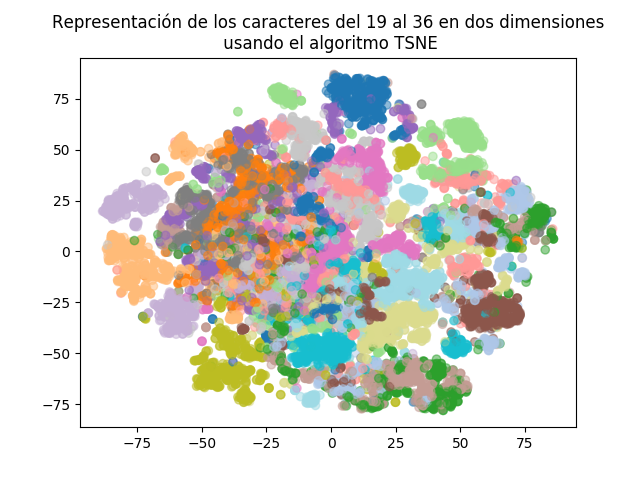
\includegraphics[width=60mm]{imgs/tsne-nopre2}}
  \caption{Proyecciones en 2D de las clases correspondientes a los caracteres del 1 al 18}
  \label{fig:char19-36}
\end{figure}

\begin{figure}[H]
  \centering
  \subfigure[PCA. Con preprocesamiento]{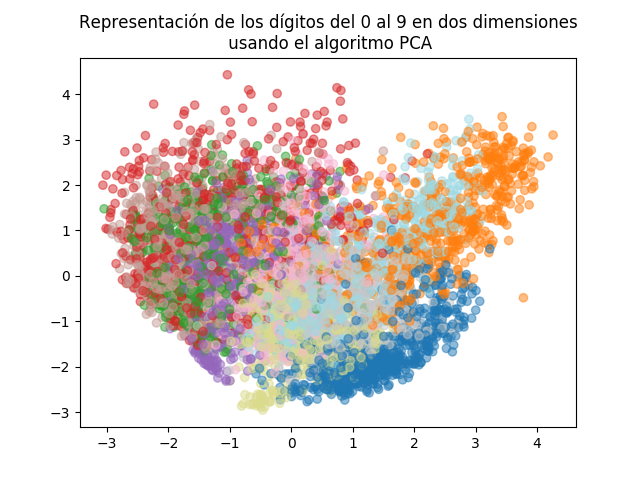
\includegraphics[width=60mm]{imgs/pca3}}
  \subfigure[PCA. Sin preprocesamiento]{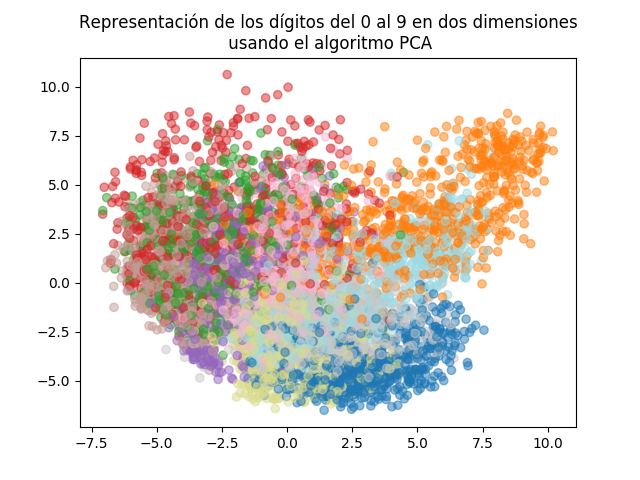
\includegraphics[width=60mm]{imgs/pca-nopre3}}
  \subfigure[TSNE. Con preprocesamiento]{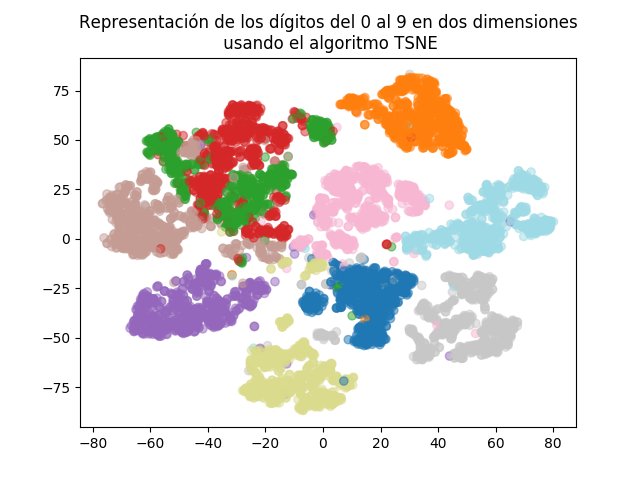
\includegraphics[width=60mm]{imgs/tsne3}}
  \subfigure[TSNE. Sin preprocesamiento]{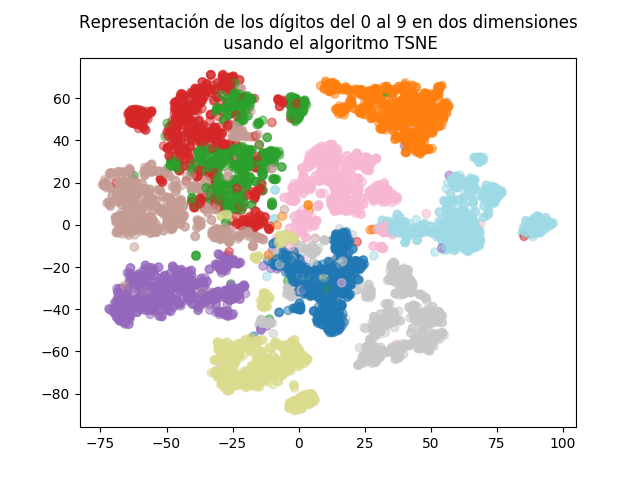
\includegraphics[width=60mm]{imgs/tsne-nopre3}}
  \caption{Proyecciones en 2D de las clases correspondientes a los caracteres del 1 al 18}
  \label{fig:digit0-9}
\end{figure}

Aunque existan algunas clases entremezcladas y algunas instancias
dispersas, en las proyecciones TSNE se percibe que los datos
correspondientes a la misma clase en general están cerca. En las
proyecciones con PCA, se distinguen ligeramente algunas clases del
resto, pero la mayoría están totalmente entremezcladas.

Comparando las proyecciones antes y después del preprocesamiento, no
parece que exista una pérdida de información significativa. Las
clases están mezcladas prácticamente en la misma medida.

No obstante, estas representaciones no deben ser nuestra única
justificación para concluir que el preprocesamiento es adecuado. Hay
que tener en cuenta que no estamos representando todas las clases en
el mismo gráfico, luego hay parejas de clases que no estamos
comparando entre sí. Es por ello y por la dificultad de interpretar el gráfico que basamos el grueso de nuestros argumentos de la sección
anterior en resultados empíricos obtenidos por validación.

\section{Modelo lineal: Regresión Logística}

Como modelo lineal elegimos Regresión Logística por ser el modelo que
mejor se adapta a clasificación multietiqueta de los que
conocemos. Este modelos viene implemendado en la función
\texttt{SGDClassifier} de \textit{sklearn}, usando como función de
pérdida la pérdida logarítmica. A la hora de predecir, este modelo
estima la probabilidad de pertenencia de una dato a cada clase y le
asigna la clase con mayor probabilidad (SoftMax).

Para intentar compensar la menor potencia de este modelo, incorporamos
algunas características polinómicas. Debido al elevado número de
variables, no incorporamos los términos cruzados (provoca error de
memoria), sólo los cuadrados, cubos y cuartas potencias de cada una de
las características originales, multiplicando el número de variables
por 4. Esto no sería viable de no haber realizado la reducción de
dimensionalidad por downsampling (provoca error de memoria). Además,
la documentación de esta función recomienda que las características
presenten varianza 1 y media 0 para una convergencia más rápida del
SGD, realizamos esto ajustando un StandardScaler (de \textit{sklearn})
a los datos de training y aplicándolo para transformar tanto éstos
como los de test.

\subsection{Estimación de hiperparámetros}

\subsection{Función de pérdida y regularización}

Dada una muestra de tamaño $N$, donde cada dato tiene $d$
características, y un problema de clasificación multietiqueta con $K$
etiquetas diferentes, la función de pérdida de este modelo es la
pérdida logarítmica:

\[ E(w_1, \ldots, w_k) = -\ln L(Y|w_1, \ldots, w_k) = -\sum\limits_{n=0}^{N}\sum\limits_{k=0}^{K} y_{nk}\ln \sigma (w^T_kx_n)\]

donde $x_n$ el vector de características de la instancia $n$-ésima,
$w_k$ es la fila $k$-ésima de una matriz de pesos $w$ de dimensión
$K \times d$ e $y_{nk} = 1$ si la instancia $n$-ésima pertenece a la
clase $k$ y $0$ en caso contrario.

La implementación de este modelo minimiza esta función de pérdida
usando gradiente descendente estocástico.

REGULARIZACIÓN


\section{Random Forest}

El modelo de random forest construye \texttt{n\_estimators} árboles de
decisión usando la totalidad de la muestra para la construcción de
cada uno, pero sólo un subconjunto de las características para
disminuir la correlación entre los árboles. Usamos la raíz cuadrada
del número de características, que es un valor adecuado según lo
estudiado en teoría y además, el valor que recomienda la
implementación de \textit{sklearn}. Tras esto, hace una media de
dichos árboles para controlar el overfitting y reducir la
variabilidad.

Elegimos este modelo por su capacidad para conseguir un bajo sesgo
combinada con una baja variabilidad. Además, los árboles de decisión
son muy adecuados para clasificación cuando el número de clases es
elevado (basta asignar una clase a cada nodo), y en nuestro caso
tenemos 46 clases.

\subsection{Estimación de hiperparámetros}

De los múltiples hiperparámetros que podríamos ajustar (profundidad
máxima de cada árbol, máximo número de nodos terminales, mínimo número
de muestras en cada nodo, \ldots), sólo buscaremos un valor adecuado
para el número de estimadores a tener en cuenta, manteniendo el resto
por defecto.

Para elegir un valor de \texttt{n\_estimators}, representamos la
accuracy media obtenida usando validación cruzada con tres
subdivisiones (hacer la media de tres ejecuciones le da cierta
estabilidad a los resultados) según diferentes valores de éste
parámetro entre $50$ y $300$. Observamos que la accuracy es
creciente con el múmero de estimadores, pero nos preguntamos si merece
la pena ese crecimiento a costa del incremento del tiempo de ejecución
que conlleva el uso de un mayor número de estimadores. Por eso,
tomamos nuevas mediciones entre $200$ y $300$, donde vimos que este
crecimiento parece saturar a partir de $275$ árboles. Así, decidimos
que el valor óptimo estaría dentro de este intervalo y repetimos ahí
el experimento, obteniendo la máxima accuracy con $290$
estimadores. Puesto que se hizo de $5$ en $5$, para obtener un valor
más exacto, tomamos mediciones cada $2$ estimadores entre $285$ y
$295$. En la cuarta gráfica, observamos dos picos, en $287$ y
$293$. Viendo la escala del eje, concluimos que la accuracy
satura en este tramo y no compensa seguir aumentando el número de
estimadores, por lo que elegimos $287$ árboles (el primer pico) como valor para el hiperparámetro.

\begin{figure}[H]
  \centering
  \subfigure[Entre $50$ y $300$, de $50$ en $50$]{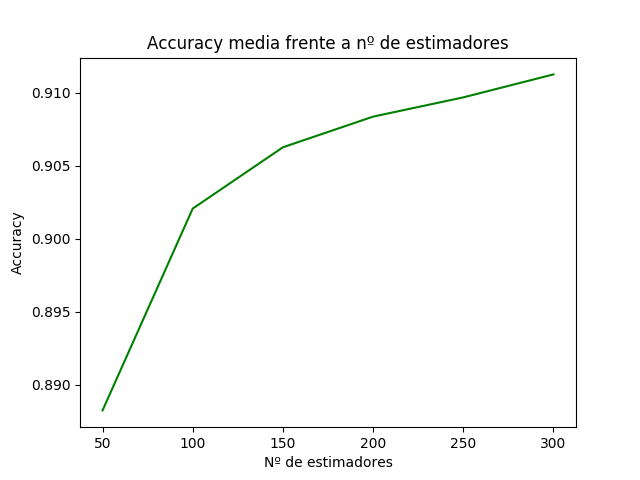
\includegraphics[width=87mm]{imgs/grafNestimators1}}
  \subfigure[Entre $200$ y $300$, de $25$ en $25$]{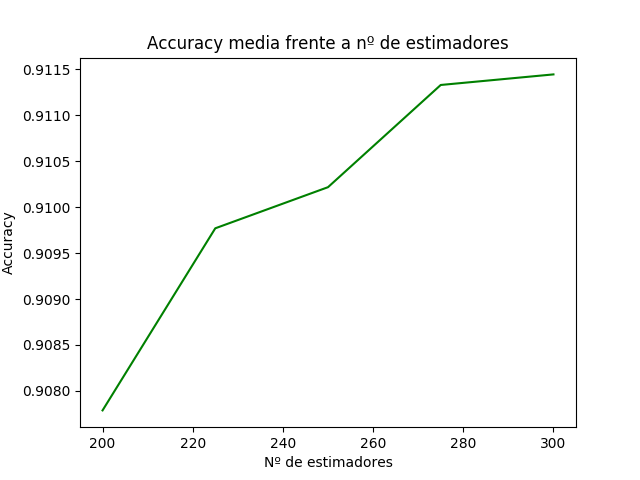
\includegraphics[width=87mm]{imgs/grafNestimators2}}
  \subfigure[Entre $275$ y $300$, de $5$ en $5$]{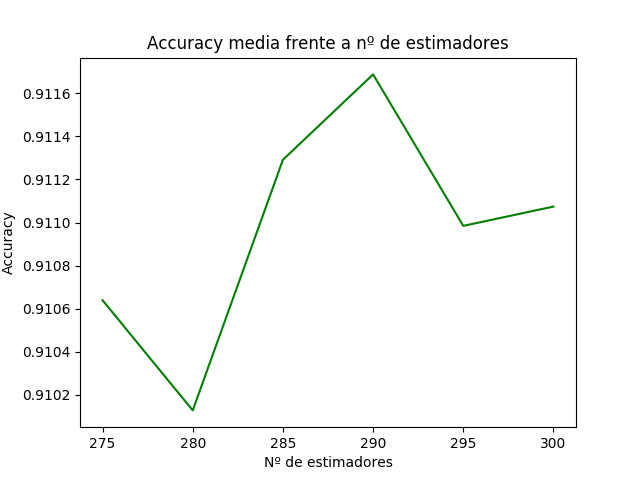
\includegraphics[width=87mm]{imgs/grafNestimators3}}
  \subfigure[Entre $285$ y $295$, de $2$ en $2$]{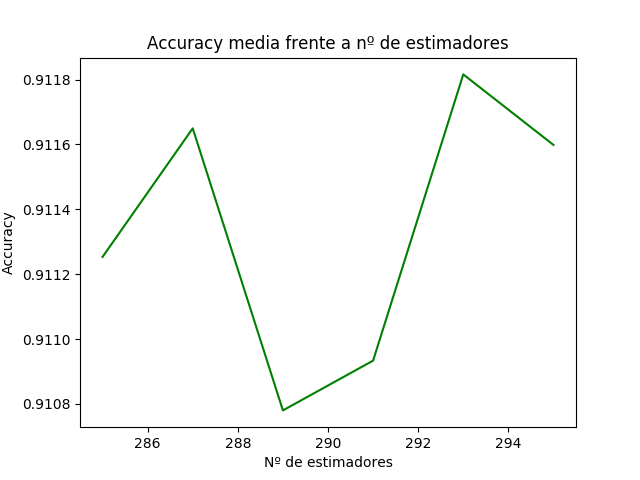
\includegraphics[width=87mm]{imgs/grafNestimators4}}
  \caption{Accuracy media de tres validaciones para distintos valores del hiperparámetro \texttt{n\_estimators}}
  \label{fig:HyperparametersRF}
\end{figure}

A continuación medimos la accuracy sobre el conjunto de train,
obteniendo $1$. Esto nos hace pensar que el modelo sobreajusta e
intentamos regularizar para reducir la complejidad (el número de
nodos) de cada árbol penalizando con el parámetro $\alpha$.

Originalmente el valor por defecto de $\alpha$ es 0, hemos probado a
incrementarlo y medir la accuracy media de tres subdivisiones de
validación cruzada para cada uno de los diferentes valores de $\alpha$
probados. Claramente, la accuracy decrece al aumentar
alpha. Observando la escala del eje en la última gráfica, concluimos
que no mejoramos nada aumentando éste, por lo que mantenemos el valor
inicial de $\alpha$, $0$.

\begin{figure}[H]
  \centering
  \subfigure[Entre $0$ y $0.0001$, $6$ mediciones]{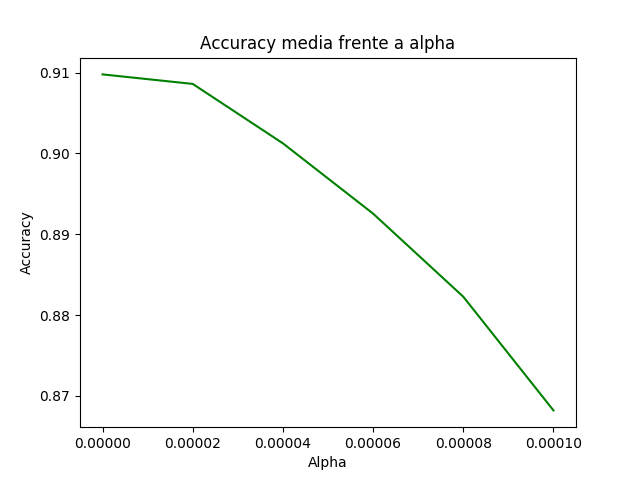
\includegraphics[width=57mm]{imgs/grafAlpha1}}
  \subfigure[Entre $0$ y $0.00005$, $11$ mediciones]{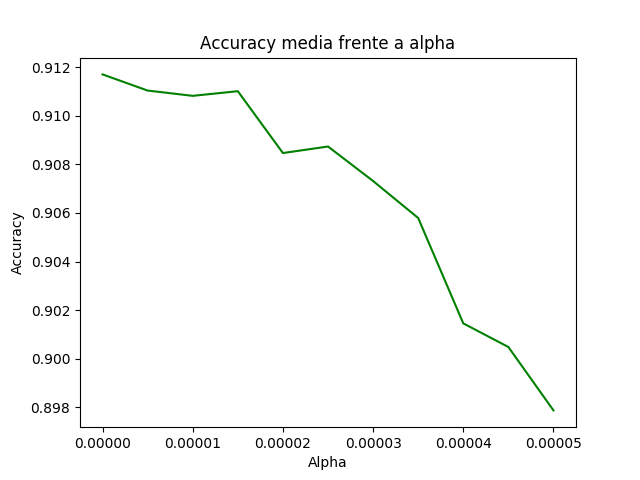
\includegraphics[width=57mm]{imgs/grafAlpha2}}
  \subfigure[Entre $0$ y $0.00001$, $6$ mediciones ]{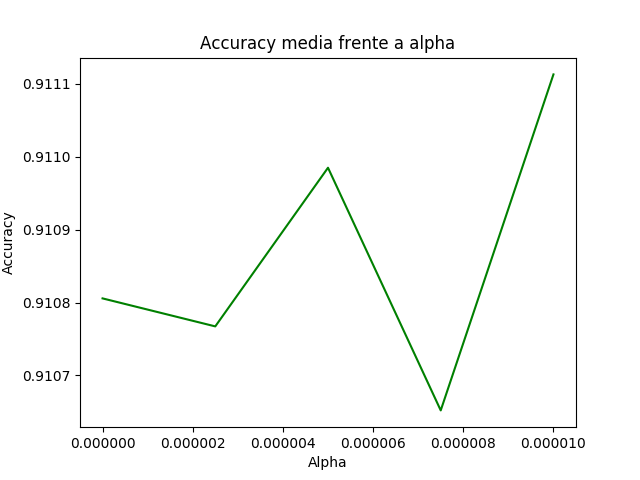
\includegraphics[width=57mm]{imgs/grafAlpha3}}
  \caption{Accuracy media de tres validaciones para distintos valores del hiperparámetro $\alpha$}
  \label{fig:HyperparametersRF}
\end{figure}

\subsection{Función de pérdida y regularización}

La función de pérdida que intenta minimizar cada uno de los árboles de
decisión que promedia random forest es:
\[R(T) = \sum\limits_{m=1}^{|T|} N_mQ_m(T) + \alpha|T|\] donde $|T|$ es el número de nodos del árbol $T$, $N_m$ es el número de instancias que caen en el nodo terminal $m$, $\alpha$ el coeficiente que penaliza la complejidad del árbol (para regularizar) y $Q_m(T)$ la medida de impureza del nodo terminal $m$. Como medida de impureza, tomamos Gini Index, aunque la entropía cruzada proporciona resultados parecidos.

La medida de impureza Gini Index es:
\[Q_m(T) = \sum\limits_{k=1}^{K} \hat p_{mk}(1 - \hat p_{mk})\] donde
$\hat p_{mk}$ es la proporción de la clase $k$ en el nodo $m$.

Como hemos visto en el apartado anterior, aumentar el valor de $\alpha$ no se consiguen mejores resultados, por lo que en este caso, a pesar de que el modelo parece sobreajustado, regularizar de esta forma no es la mejor opción. Es por esto que tomamos $\alpha = 0$, quedando la función de pérdida:
\[R(T) = \sum\limits_{m=1}^{|T|} N_mQ_m(T)\]

\section{Multilayer Perceptron (MLP)}

El modelo de perceptrón multicapa usado consta de tres capas: la capa
de entrada, dos ocultas y una de salida. Como función de activación en
cada neurona hemos considerado $\tanh$ y como algoritmo para ajustar
los pesos usamos Adam, como nos recomendaron en teoría y como
recomienda la documentación de \textit{sklearn} para datasets grandes
como es el nuestro.

Al igual que random forest, el perceptrón multicapa tiene suficiente
complejidad para obtener un bajo sesgo y facilidad para clasificación
no binaria. Para afrontar el problema del sobreajuste, podemos
utilizar early stopping como regularización, ya que disponemos de un
número elevado de muestras de entrenamiento y podemos permitirnos
sacrificar algunas con el fin de combatir el sobreajuste. Por tanto,
consideramos este modelo adecuado para el problema.

\subsection{Estimación de hiperparámetros}

Estimamos el número de neuronas, \texttt{N\_NEUR}, que tiene cada una
de las capas ocultas. Como nos recomendaban valores entre $50$ y $100$
hicimos las mediciones de la accuracy media usando validación cruzada
con dos subdivisiones del modelo con \texttt{N\_NEUR} en dicho
rango. Observamos que el máximo se alcanza en torno a $60$ neuronas
por capa, luego repetimos las mediciones ahora en el intervalo
$[55,70]$. A pesar de que la diferencia entre la accuracy es leve,
seguimos buscando un valor para \texttt{N\_NEUR} en torno a $60$, que
es donde conseguimos la accuracy más alta. Al medir la accuracy en el
intervalo $[58,62]$, obtenemos el máximo en $59$. Por tanto, cada capa
oculta del MLP usado para el ajuste tendrá 59 neuronas.

\begin{figure}[H]
  \centering
  \subfigure[Entre $50$ y $100$, de $10$ en $10$]{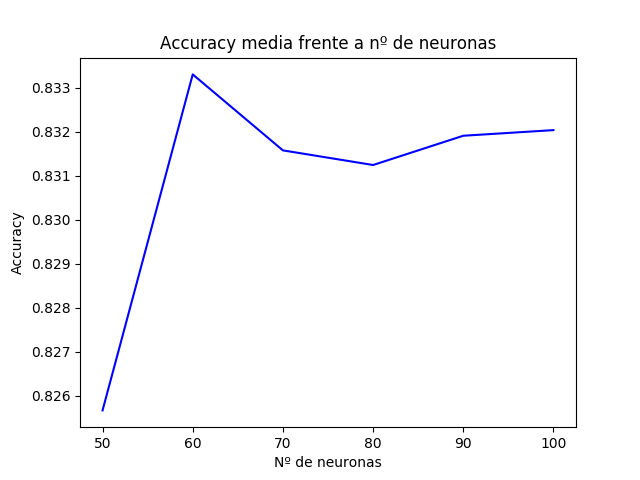
\includegraphics[width=57mm]{imgs/grafNneur1}}
  \subfigure[Entre $55$ y $70$, de $5$ en $5$]{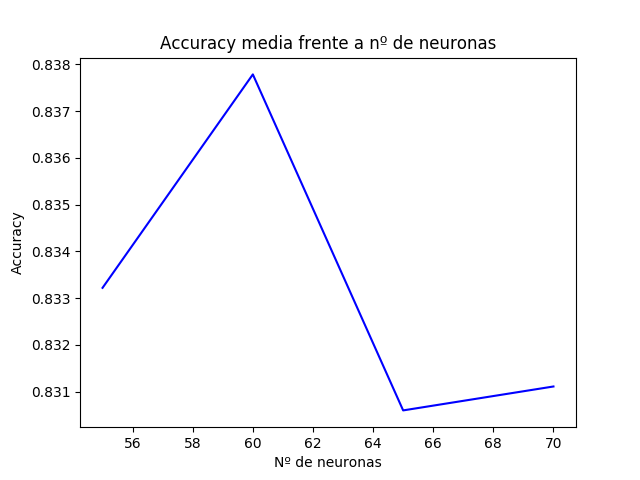
\includegraphics[width=57mm]{imgs/grafNneur2}}
  \subfigure[Entre $58$ y $62$, de $1$ en $1$ ]{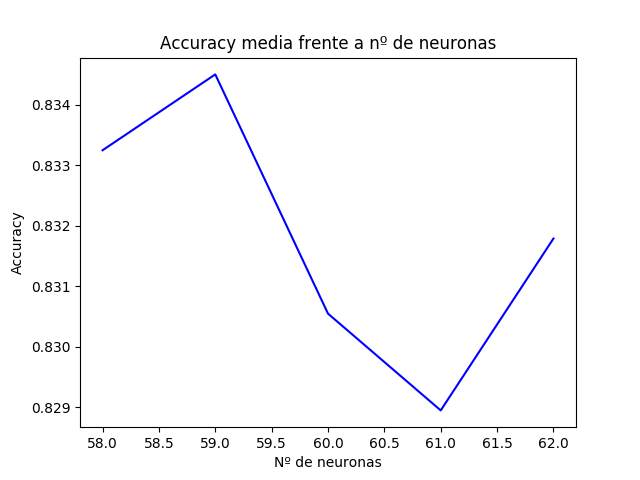
\includegraphics[width=57mm]{imgs/grafNneur3}}
  \caption{Accuracy media de dos validaciones para distintos valores del hiperparámetro \texttt{N\_NEUR}}
  \label{fig:HyperparametersRF}
\end{figure}

\subsection{Función de pérdida y regularización}

En la documentación nos indican que la función de pérdida usada en la
implementación de \texttt{MLPClassifier} es la pérdida logarítmica,
que para clasificación multietiqueta, con un conjunto de $K$
etiquetas, es:

\[ L_{\log}(Y,P) = -\log Pr(Y|P) = -\frac{1}{N}\sum\limits_{i=0}^{N-1}\sum\limits_{k=0}^{K-1} y_{ik}\log p_{ik}\]

donde $Y$ es uma matriz codificada en binario con las verdaderas
etiquetas de la muestra, es decir, $y_{ik} = 1$ si el dato $x_i$ tiene
etiqueta $k$ (y $0$ en otro caso) y $P$ es una matriz de estimaciones
probabilísticas que depende de los pesos.

Para regularizar usamos Early Stopping (\texttt{early\_stopping =
  True}). Esto separa un 10\% de los datos de ajuste para validación y
termina el entrenamiento cuando la accuracy de este conjunto no mejora
en al menos $10^{-4}$ por 10 iteraciones consecutivas.

%Meter resultados

\end{document}
